% -*- root: ../mainThesis.tex -*-
\chapter{Results and numerical tests} 
In this chapter we present the results of the implementations
of the well distance projection and the inter-well distance 
projection and the alternating projection method applied to the
joint problem. We also include numerical results from the computations
of well indices and compare them to the results found using 
the reservoir simulator RMS. Figures are also supplied whenever
possible. 
%
\section{Well constraint projections}
%
For all projections in this section we set the well length constraint 
(i.e., shortest and longest wells allowed) and inter-well distance 
constraint (i.e., the minimum distance required to be between all 
pairs of wells) parameters to the following values:
%
\begin{align}
L_{\min} &= 5,  \\
L_{\max} &= 10, \\
d &= 4.
\label{eq:constraint_parameters}
\end{align}
%
This means that in the final configuration all wells must have a 
length between 5 and 10, and no two wells are allowed to be 
closer than a distance 4 to each other.
%
The well length projection was tested on a single well and 
simultaneously on a set of five wells. the inter-well distance 
projection was tested on two wells and then as an alternating projection
on five wells. Both projections were then applied alternatingly on one
set of two wells and one set of five wells until a feasible solution was 
reached.
%
\subsection{Well length projection}
%
%
\paragraph{Well length constraint on a single well}
%
First consider the well with endpoints $(-\frac{1}{2},0,\frac{1}{2})$
and $(\frac{1}{2},0,\frac{1}{2})$. This well has length 2 and its length
is increased as shown in Figure \ref{fig:trivial_min}.
%
\begin{figure}[H]
	\centering
	\begin{subfigure}{0.44\textwidth}
		\centering
		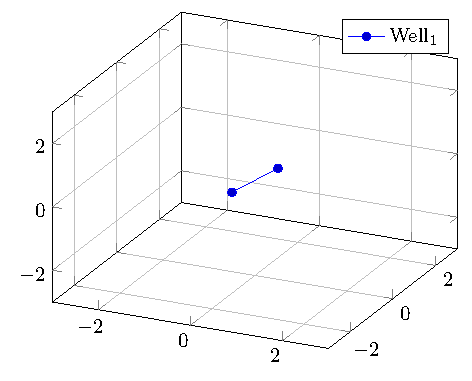
\includegraphics[width=1\textwidth]{figures/trivial_projections/trivial_initial.pdf}
		\caption{Initial well. The well has length 2 and violates the well length constraint
				  because it is too short.}
		\label{fig:trivial_min_a}
	\end{subfigure}\hfill
	\hspace{.05\linewidth}
	\begin{subfigure}{0.44\textwidth}
		\centering
		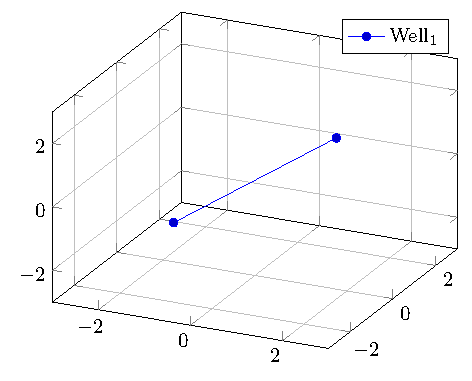
\includegraphics[width=1\textwidth]{figures/trivial_projections/trivial_min.pdf}
		\caption{The well has been projected to satisfy the well length length constraint.
				  The projected well has length 5 which is equal to $L_{\min}$.}
		\label{fig:trivial_min_b}
	\end{subfigure}
	\caption{The well on the left that violates the well length constraint
			 has been projected to a feasible solution on the right.}
	\label{fig:trivial_min}
\end{figure}
%
%
Now consider the well with endpoints $(-5,-5,-5)$,
$(5,5,5)$. This well has length $10\sqrt{3}$ and its length
is decreased as shown in Figure \ref{fig:trivial_max}.
%
\begin{figure}[H]
	\centering
	\begin{subfigure}{0.44\textwidth}
		\centering
		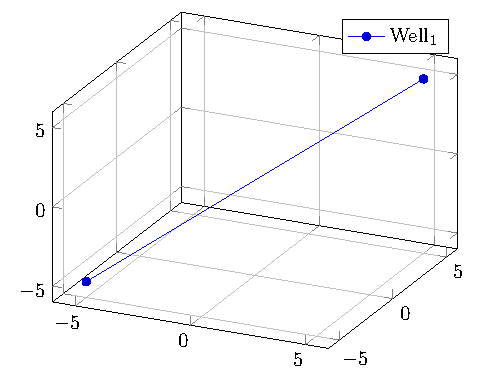
\includegraphics[width=1\textwidth]{figures/trivial_projections/trivial_initial_max.pdf}
		\caption{Initial well. The well has length $10\sqrt{3}$ and violates the well length constraint
				  because it is too long.}
	\end{subfigure}\hfill
	\hspace{.05\linewidth}
	\begin{subfigure}{0.44\textwidth}
		\centering
		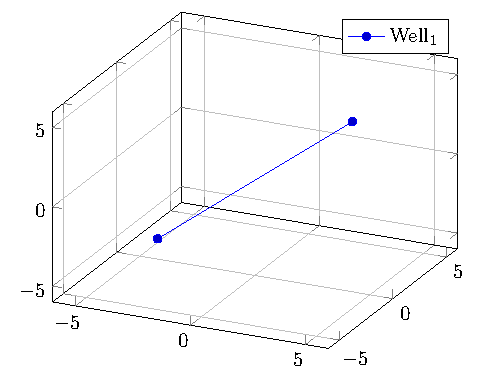
\includegraphics[width=1\textwidth]{figures/trivial_projections/trivial_max.pdf}
		\caption{The well has been projected to satisfy the well length length constraint.
				  The projected well has length 10 which is equal to $L_{\max}$.}
	\end{subfigure}
	\caption{The well on the left that violates the well length constraint
			 has been projected to a feasible solution on the right.}
	\label{fig:trivial_max}
\end{figure}
%
Lastly five wells were were created as shown in Figure \ref{fig:initial_5_well}.
%
\begin{figure}[H]
	\centering
	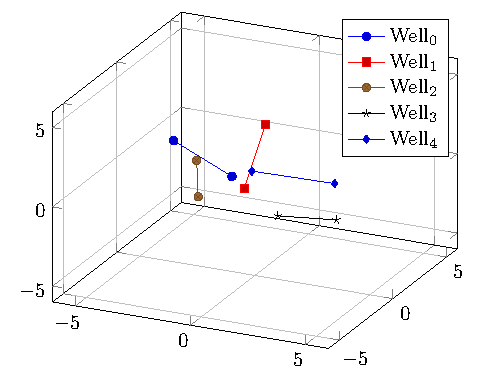
\includegraphics[width=0.70\textwidth]{figures/interwell_distance/five_wells.pdf}
	\caption{Initial positions of five wells. Both the well distance constraint and the
											  inter-well distance constraint are violated
											  by one or more wells.}
	\label{fig:initial_5_well}
\end{figure}
%
Note that since the well lenghts are independent from
each other the well lenght projection of multiple wells is
eqivalent to sequential projection of single wells.
In Figure \ref{fig:initial_5_well_length} we can see the
five well length projections.
%
\begin{figure}[H]
	\centering
	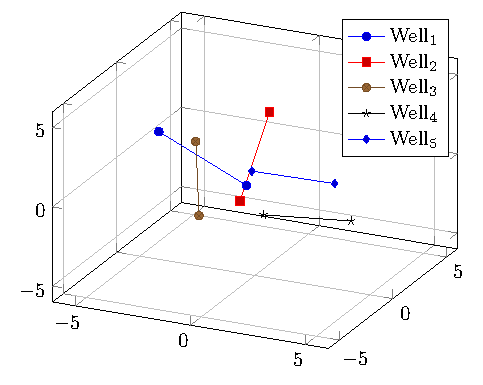
\includegraphics[width=0.70\textwidth]{figures/well_length/well_length_moved.pdf}
	\caption{Well length projection on five wells. Five wells have been moved so that the well
										length constraint is satisfied for all wells.
										The inter-well distance constraint however is
										not satisfied.}
	\label{fig:initial_5_well_length}
\end{figure}
%
\subsection{Inter-well distance projection}
%
The inter-well distance projection was first tested on two wells,
$\text{Well}_1$ and $\text{Well}_2$, with initial coordinates 
%
\begin{align*}
\text{Well}_1 = \left( (-1,0,0), (0,1,0) \right) \quad \text{and} \quad  \text{Well}_2 = \left( (0,-1,0), (1,0,0) \right).
\end{align*}
%
Note that the wells in this case are parallel and, as
mentioned in Section 3.2.1, there is no unique shortest 
distance line between the two wells. Still the numerical
solution is found and the resulting four-point solution 
can be seen in Figure \ref{fig:trivial_interwell_1}.
%
\begin{figure}[H]
	\centering
	\begin{subfigure}{0.44\textwidth}
		\centering
		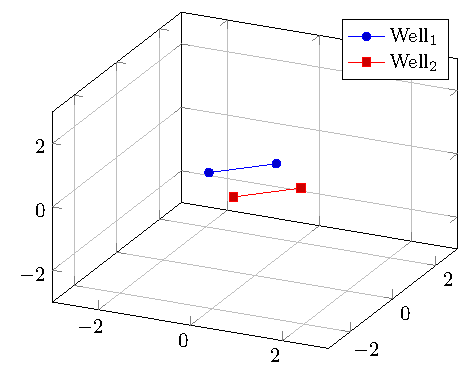
\includegraphics[width=1\textwidth]{figures/interwell_distance_two_wells/initial.pdf}
		\caption{Initial wells. The shortest distance between the wells is $\sqrt{2}$ which is
								 less than $d=4$, and thus the inter-well distance constraint is
								 violated.}
	\end{subfigure}\hfill
	\hspace{.05\linewidth}
	\begin{subfigure}{0.44\textwidth}
		\centering
		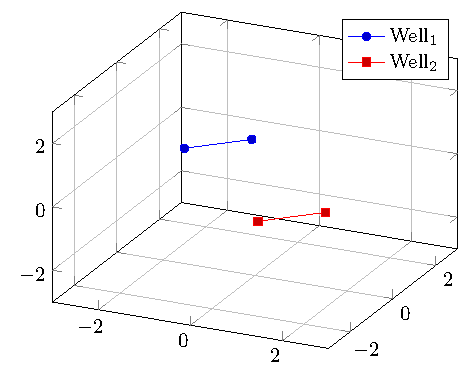
\includegraphics[width=1\textwidth]{figures/interwell_distance_two_wells/initial_moved.pdf}
		\caption{The wells have been moved so the the shortest distance between them is 4.}
	\end{subfigure}
	\caption{The wells initial positions don't satisfy the inter-well distance constraint. The wells
						are moved so that the shortest distance between them is exactly equal to $d = 4$.}
	\label{fig:trivial_interwell_1}
\end{figure}
%
The inter-well distance projection was then tested on two 
wells $\text{Well}_3$ and $\text{Well}_4$, with initial
coordinates 
%
\begin{align*}
\text{Well}_3 = \left( (-2,-2,0), (-2,2,0) \right) \quad \text{and} \quad  \text{Well}_4 = \left( (0,0,0), (3,0,0) \right).
\end{align*}
%
The point to the right on $\text{Well}_4$ is exactly a distance 4 away from $\text{Well}_3$,
but clearly the points of $\text{Well}_3$ will be moved to the left, so we expect the right
point on $\text{Well}_4$ to remain static. Indeed the projection, which is shown in Figure
\ref{fig:trivial_interwell_2} only moves 3 points, and we have a three-point solution.
%
\begin{figure}[H]
	\centering
	\begin{subfigure}{0.44\textwidth}
		\centering
		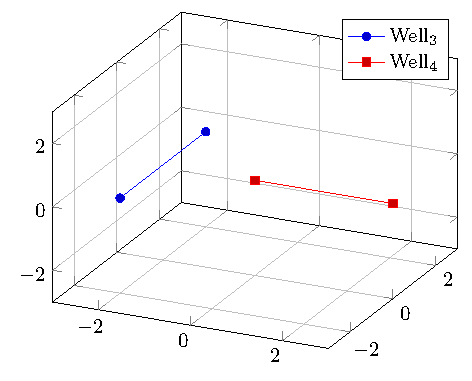
\includegraphics[width=1\textwidth]{figures/interwell_distance_two_wells/initial_2.pdf}
		\caption{Initial wells. The shortest distance between the wells is 1 which is
								 less than $d=4$, and thus the inter-well distance constraint is
								 violated.}
	\end{subfigure}%\hfill
	\hspace{.05\linewidth}
	\begin{subfigure}{0.44\textwidth}
		\centering
		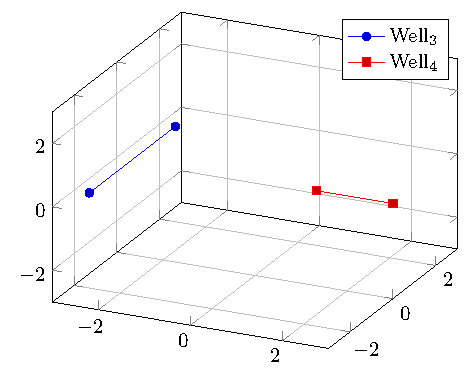
\includegraphics[width=1\textwidth]{figures/interwell_distance_two_wells/initial_2_moved.pdf}
		\caption{The wells have been moved so the the shortest distance between them is 4.}
	\end{subfigure}%
	\caption{The wells initial positions don't satisfy the inter-well distance constraint. The wells
						are moved so that the shortest distance between them is exactly equal to $d = 4$.
						The point to the right on $\text{Well}_4$ is not moved at all, which means this
						is a three-point solution as discussed in Chapter 3.}
	\label{fig:trivial_interwell_2}
\end{figure}
%
We refer to Chapter 8 for discussion on a single projection that failed.
%
\subsection{Alternating projections to joint problem}
%
We start with alternating projections on two wells with initial
coordinates $\left( (-2,-2,0), (-2,2,0) \right)$ and $\left( (0,0,0), (3,0,0) \right)$
as seen in Figure \ref{fig:alternate_two_a}. The resulting position in Figure 
\ref{fig:alternate_two_b} took 8 alternating iterations to be reached. 

%
\begin{figure}[H]
	\centering
	\begin{subfigure}{0.44\textwidth}
		\centering
		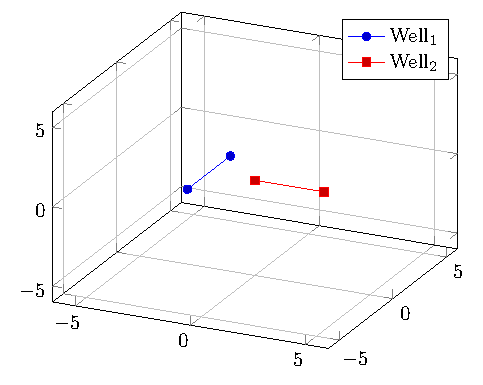
\includegraphics[width=1\textwidth]{figures/both_projections/two_wells_initial.pdf}
		\caption{Initial wells. The shortest distance between the wells is 1 which is
								 less than $d=4$, and thus the inter-well distance constraint is
								 violated.}
		\label{fig:alternate_two_a}
	\end{subfigure}%\hfill
	\hspace{.05\linewidth}
	\begin{subfigure}{0.44\textwidth}
		\centering
		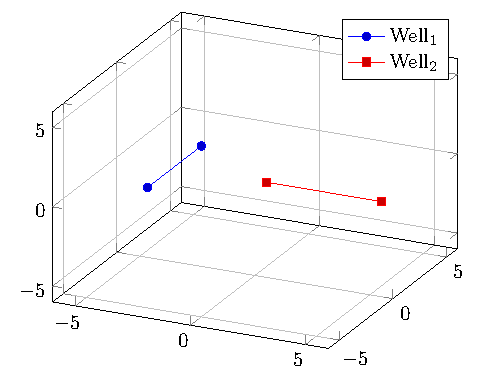
\includegraphics[width=1\textwidth]{figures/both_projections/two_wells_moved.pdf}
		\caption{The wells have been moved so the the shortest distance between them is 4 and
				 the lengths of the wells have been adjusted.}
		\label{fig:alternate_two_b}
	\end{subfigure}%
	\caption{The wells initial positions don't satisfy the inter-well distance constraint. The wells
						are moved so that the shortest distance between them is exactly equal to $d = 4$.
						The point to the right on $\text{Well}_4$ is not moved at all, which means this
						is a three-point solution as discussed in Chapter 3.}
	\label{fig:alternate_two}
\end{figure}
%
Actually the constraints are never fully satisfied in this case because
the projections work against each other. We have implemented a tolerance
for accepting a position as feasible, but in this case we can get arbitrarily
close to a feasible solution given enough iterations.
%

Now the five wells seen in Figure \ref{fig:initial_5_well} 
are projected using alternating projections. Theoretically 
there is no guarantee that any of the projections will
converge.
%
First we use the inter-well distance projection on pairs
of wells until a feasible solution is reached. After iterating
four times over all pairs of wells the solution in Figure
\ref{fig:initial_5_well_distance} was found.
%
\begin{figure}[H]
	\centering
	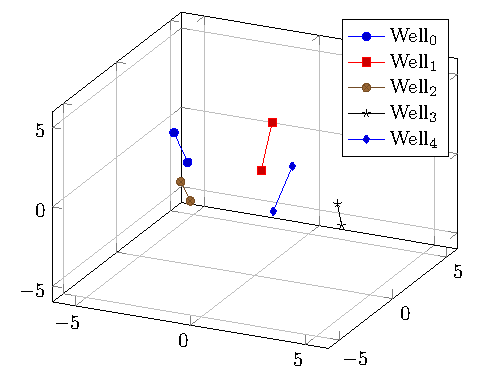
\includegraphics[width=0.70\textwidth]{figures/interwell_distance/five_wells_moved.pdf}
	\caption{Inter-well distance projection on five wells. By running inter-well projection on 
											 wells pairwise, the five wells have been moved so 
											 that the inter-well distance constraint is satisfied 
											 for all pairs of wells. The Solution took four steps of 
											 iterating over all pairs. The well length constraint 
											 is not satisfied for any of the wells because they
											 are all too short. This is not surprising because the inter-well
											 distance projection can only shorten the length of a well.}
	\label{fig:initial_5_well_distance}
\end{figure}
%
%
Finally both projections were done alternatingly until
the five wells satisfied both constraints. The final
positions of the wells, which can be seen in Figure 
\ref{fig:initial_5_both}, was found after six iterations
of each projection. Again the solution is not feasible
but the error is sufficiently small to stop the iterations.
%
\begin{figure}[H]
	\centering
	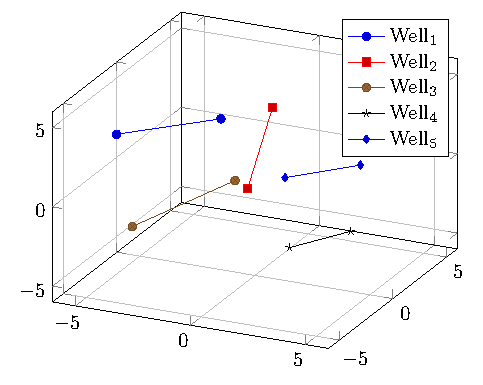
\includegraphics[width=0.70\textwidth]{figures/both_projections/both_projections.pdf}
	\caption{Alternating well length- and inter-well distance projection. By alternating between
											well length projection and inter-well distance projection
											the wells have been moved so that the well length constraint
											is satisfied for all wells and the inter-well distance constraint
											is satisfied for all pairs of wells. The solution took six 
											steps of alternating projections.}
	\label{fig:initial_5_both}
\end{figure}
%
%
\section{Well index calculation}
%
We use a reservoir containing $60 \times 60$ well blocks with
dimensions $\Delta_x = \Delta_y = \Delta_z = 24$ and varying 
permeabilities. We ran the intersecting well blocks and well 
index calculation algorithms on a well with wellbore radius
$r_w = \frac{0.1905}{2}$,
which runs from the middle of the block located in the bottom
left corner and straight to the block in the bottom right corner
as indicated by Figure \ref{fig:well_intersection}.
%
\begin{figure}[H]
	\centering
	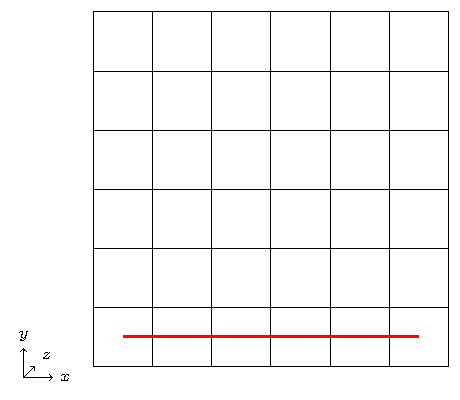
\includegraphics[width=0.40\textwidth]{figures/well_index/well_intersection.pdf}
	\caption{Well that goes from block 0 in the bottom left corner and ends up
	in block 59 in the bottom right corner. For illustration purposes the figure has been edited and every 
	square actually contains 10 $\times$ 10 blocks}
	\label{fig:well_intersection}
\end{figure}
%
The calculated well indices from the first few well
blocks of our implementation and the results obtained 
from RMS can be seen in Table \ref{tab:well_indexes}. 
%
\begin{center}
	\captionof{table}{Computed well indices compared to the well indices calculated by RMS}
	\begin{tabular}[h]{ccc}
	Block number & Well index (Our algorithm) & Well index (RMS) \\
	\hline
	\hline
	0 & 0.213273 & 0.21327 \\
	1 & 0.328879 & 0.32888 \\
	2 & 0.328879 & 0.32888 \\ 
	3 & 0.501907 & 0.50191 \\
	4 & 0.471228 & 0.47123 \\
	5 & 0.593556 & 0.59356 \\
	6 & 0.924533 & 0.92453 \\
	7 & 1.287440 & 1.28744 \\
	8 & 0.905511 & 0.90551
	\label{tab:well_indexes}
	\end{tabular}
\end{center}
%
%
